%%**************************************************************
%% Vorlage fuer Bachelorarbeiten (o.ä.) der DHBW
%%
%% Autor: Tobias Dreher, Yves Fischer, Michael Gruben, Markus Barthel
%% Datum: 06.07.2011 - 22.08.2014
%% 
%% Autor: Ferdinand König und Maximilian Köhler
%% Datum: 2020 - 2022
%%**************************************************************

%!TEX root = ../main.tex

%
% Nahezu alle Einstellungen koennen hier getaetigt werden
%

\RequirePackage[l2tabu, orthodox]{nag}	% weist in Commandozeile bzw. log auf veraltete LaTeX Syntax hin

\documentclass[%
    final,
	pdftex,
	oneside,			% Einseitiger Druck (oneside) oder zweiseitig (twoside)
	headings=openright,	% Kapitelanfänge immer auf rechter Seite (bei zweiseitig)
	cleardoublepage=empty,	% Leere Vakatseiten
	12pt,				% Schriftgroesse
	parskip=half,		% Halbe Zeile Abstand zwischen Absätzen (half).
%	topmargin = 10pt,	% Abstand Seitenrand (Std:1in) zu Kopfzeile [laut log: unused]
	headheight = 20pt,	% Höhe der Kopfzeile
%	headsep = 30pt,	% Abstand zwischen Kopfzeile und Text Body  [laut log: unused]
	headsepline,		% Linie nach Kopfzeile.
	footsepline,		% Linie vor Fusszeile.
	footheight = 20pt,	% Höhe der Fusszeile
	abstracton,		% Abstract Überschriften
	DIV=calc,		% Satzspiegel berechnen
	BCOR=0mm,		% Bindekorrektur links: 8mm
	headinclude=false,	% Kopfzeile nicht in den Satzspiegel einbeziehen
	footinclude=false,	% Fußzeile nicht in den Satzspiegel einbeziehen
	listof=totoc,		% Abbildungs-/ Tabellenverzeichnis im Inhaltsverzeichnis darstellen
	toc=bibliography,	% Literaturverzeichnis im Inhaltsverzeichnis darstellen
	pointlessnumbers,
	% bibliography=openstyle
]{scrreprt}	% Koma-Script report-Klasse, fuer laengere Bachelorarbeiten alternativ auch: scrbook

\raggedbottom

% Einstellungen laden
\usepackage{xstring}
\usepackage[utf8]{inputenc}
\usepackage[T1]{fontenc}

\newcommand{\einstellung}[1]{%
  \expandafter\newcommand\csname #1\endcsname{}
  \expandafter\newcommand\csname setze#1\endcsname[1]{\expandafter\renewcommand\csname#1\endcsname{##1}}
}
\newcommand{\langstr}[1]{\einstellung{lang#1}}

\einstellung{matrikelnr}
\einstellung{titel}
\einstellung{kurs}
\einstellung{datumAbgabe}
\einstellung{firma}
\einstellung{firmenort}
\einstellung{abgabeort}
\einstellung{abschluss}
\einstellung{studiengang}
\einstellung{dhbw}
\einstellung{betreuer}
\einstellung{gutachter}
\einstellung{zeitraum}
\einstellung{arbeit}
\einstellung{autor}
\einstellung{sprache}
\einstellung{schriftart}
\einstellung{seitenrand}
\einstellung{kapitelabstand}
\einstellung{spaltenabstand}
\einstellung{zeilenabstand}
\einstellung{zitierstil}
 % verfügbare Einstellungen
%%%%%%%%%%%%%%%%%%%%%%%%%%%%%%%%%%%%%%%%%%%%%%%%%%%%%%%%%%%%%%%%%%%%%%%%%%%%%%%
%                                   Einstellungen
%
% Hier können alle relevanten Einstellungen für diese Arbeit gesetzt werden.
% Dazu gehören Angaben u.a. über den Autor sowie Formatierungen.
%%%%%%%%%%%%%%%%%%%%%%%%%%%%%%%%%%%%%%%%%%%%%%%%%%%%%%%%%%%%%%%%%%%%%%%%%%%%%%%


%%%%%%%%%%%%%%%%%%%%%%%%%%%%%%%%%%%% Sprache %%%%%%%%%%%%%%%%%%%%%%%%%%%%%%%%%%%
%% Aktuell sind Deutsch und Englisch unterstützt.
%% Es werden nicht nur alle vom Dokument erzeugten Texte in
%% der entsprechenden Sprache angezeigt, sondern auch weitere
%% Aspekte angepasst, wie z.B. die Anführungszeichen und
%% Datumsformate.
\setzesprache{de} % de oder en
%%%%%%%%%%%%%%%%%%%%%%%%%%%%%%%%%%%%%%%%%%%%%%%%%%%%%%%%%%%%%%%%%%%%%%%%%%%%%%%%



%%%%%%%%%%%%%%%%%%%%%%%%%%%%%%%%%%% Angaben  %%%%%%%%%%%%%%%%%%%%%%%%%%%%%%%%%%%
%% Die meisten der folgenden Daten werden auf dem
%% Deckblatt angezeigt, einige auch im weiteren Verlauf
%% des Dokuments.
\setzematrikelnr{XXXXXXX}
\setzekurs{TMB19 AM2}
\setzetitel{Studienarbeitstitel}
\setzedatumAbgabe{19. September 2022}
\setzefirma{Beispielfirma}
\setzefirmenort{Beispieladresse, XXXXX Beispielort}
\setzeabgabeort{Mannheim}
\setzestudiengang{Maschinenbau}
\setzedhbw{Mannheim}
\setzebetreuer{Herr XY}
\setzegutachter{Frau XY}
\setzezeitraum{27.06.2022\ -\ 19.09.2022}
\setzearbeit{Studienarbeit}
\setzeautor{Max Mustermann}




%%%%%%%%%%%%%%%%%%%%%%%%%%%% Literaturverzeichnis %%%%%%%%%%%%%%%%%%%%%%%%%%%%%%
%% Bei Fehlern während der Verarbeitung bitte in ads/header.tex bei der
%% Einbindung des Pakets biblatex (ungefähr ab Zeile 110,
%% einmal für jede Sprache), biber in bibtex ändern.
\newcommand{\ladeliteratur}{%
\addbibresource{bibliographie.bib}
%\addbibresource{weitereDatei.bib}
}
%% Zitierstil
%% siehe: http://ctan.mirrorcatalogs.com/macros/latex/contrib/biblatex/doc/biblatex.pdf (3.3.1 Citation Styles)
%% mögliche Werte z.B numeric-comp, alphabetic, authoryear, numeric
\setzezitierstil{numeric-comp}
%\setzezitierstil{alphabetic}
%\setzezitierstil{authoryear}




%%%%%%%%%%%%%%%%%%%%%%%%%%%%%%%%% Layout %%%%%%%%%%%%%%%%%%%%%%%%%%%%%%%%%%%%%%%
%% Verschiedene Schriftarten
% laut nag Warnung: palatino obsolete, use mathpazo, helvet (option scaled=.95), courier instead
\setzeschriftart{lmodern} % palatino oder goudysans, lmodern, libertine, mathptmx
% palatino oder lmodern ganz nett

%% Paket um Textteile drehen zu können
%\usepackage{rotating}
%% Paket um Seite im Querformat anzuzeigen
%\usepackage{lscape}

%% Seitenränder
% \setzeseitenrand{2.5cm}

%% Abstand vor Kapitelüberschriften zum oberen Seitenrand
\setzekapitelabstand{0pt}

%% Spaltenabstand
\setzespaltenabstand{10pt}
%%Zeilenabstand innerhalb einer Tabelle
\setzezeilenabstand{1.5}




%%%%%%%%%%%%%%%%%%%%%%%%%%%%% Verschiedenes  %%%%%%%%%%%%%%%%%%%%%%%%%%%%%%%%%%%
%% Farben (Angabe in HTML-Notation mit großen Buchstaben)
\newcommand{\ladefarben}{%
	\definecolor{LinkColor}{HTML}{00007A}
	\definecolor{ListingBackground}{HTML}{FCF7DE}
}

%%Mathematikpakete benutzen (Pakete aktivieren)
\usepackage{amsmath}
\usepackage{amssymb}

%% Programmiersprachen Highlighting (Listings)
\newcommand{\listingsettings}{%
	\lstset{%
		language=Java,			% Standardsprache des Quellcodes
		numbers=left,			% Zeilennummern links
		stepnumber=1,			% Jede Zeile nummerieren.
		numbersep=5pt,			% 5pt Abstand zum Quellcode
		numberstyle=\tiny,		% Zeichengrösse 'tiny' für die Nummern.
		breaklines=true,		% Zeilen umbrechen wenn notwendig.
		breakautoindent=true,	% Nach dem Zeilenumbruch Zeile einrücken.
		postbreak=\space,		% Bei Leerzeichen umbrechen.
		tabsize=2,				% Tabulatorgrösse 2
		basicstyle=\ttfamily\footnotesize, % Nichtproportionale Schrift, klein für den Quellcode
		showspaces=false,		% Leerzeichen nicht anzeigen.
		showstringspaces=false,	% Leerzeichen auch in Strings ('') nicht anzeigen.
		extendedchars=true,		% Alle Zeichen vom Latin1 Zeichensatz anzeigen.
		captionpos=b,			% sets the caption-position to bottom
		backgroundcolor=\color{ListingBackground}, % Hintergrundfarbe des Quellcodes setzen.
		xleftmargin=0pt,		% Rand links
		xrightmargin=0pt,		% Rand rechts
		frame=single,			% Rahmen an
		frameround=ffff,
		rulecolor=\color{darkgray},	% Rahmenfarbe
		fillcolor=\color{ListingBackground},
		keywordstyle=\color[rgb]{0.133,0.133,0.6},
		commentstyle=\color[rgb]{0.133,0.545,0.133},
		%stringstyle=\color[rgb]{0.627,0.126,0.941}
		stringstyle=\color{red}
	}
}




%%%%%%%%%%%%%%%%%%%%%%%%%%%%%%%% Eigenes %%%%%%%%%%%%%%%%%%%%%%%%%%%%%%%%%%%%%%%
%% Hier können Ergänzungen zur Präambel vorgenommen werden (eigene Pakete, Einstellungen)

%colorpackage
% \usepackage{color}
\usepackage[table]{xcolor}


%listing package for defining new language
\usepackage{listings}

% starting footnotes at 1
% \usepackage{perpage}
% \MakePerPage[1]{footnote}

%Functions
\def\bsq#1{%both single quotes
\lq{#1}\rq}


%%%%%%%%%%%%%%%%%%%%%%%%%%%%%%%%%%%%%%%%%%%%
% selfmade language pakets
% JavaScript language
\definecolor{lightgray}{RGB}{227, 227, 227}
\definecolor{darkgray}{RGB}{100, 100, 100}
\definecolor{purple}{rgb}{0.65, 0.12, 0.82}
\definecolor{schaeffler}{RGB}{0, 137, 61}
\definecolor{dark-green}{RGB}{0, 110, 93}
\definecolor{middle-green}{RGB}{115, 161, 149}
\definecolor{light-green}{RGB}{199, 222, 160}

\definecolor{pie1}{RGB}{115, 161, 149}
\definecolor{pie2}{RGB}{192, 198, 191}
\definecolor{pie3}{RGB}{135, 135, 135}
\definecolor{pie4}{RGB}{29, 155, 178}
\definecolor{pie5}{RGB}{182, 186, 194}
\definecolor{pie6}{RGB}{161, 200, 97}
\definecolor{pie7}{RGB}{67, 99, 91}
\definecolor{pie8}{RGB}{112, 123, 110}
\definecolor{pie9}{RGB}{113, 113, 113}

% \lstdefinelanguage{style-js}{
%   keywords={break, case, catch, continue, debugger, default, delete, do, else, false, finally, for, function, if, in, instanceof, new, null, return, switch, this, throw, true, try, typeof, var, void, while, with},
%   morecomment=[l]{//},
%   morecomment=[s]{/*}{*/},
%   morestring=[b]',
%   morestring=[b]",
%   ndkeywords={class, export, boolean, throw, implements, import, this},
%   keywordstyle=\color{blue}\bfseries,
%   ndkeywordstyle=\color{darkgray}\bfseries,
%   identifierstyle=\color{black},
%   commentstyle=\color[rgb]{0.133,0.545,0.133},
%   %commentstyle=\color{purple}\ttfamily,
%   stringstyle=\color{red}\ttfamily,
%   sensitive=true
% }

% Einstellung für die Einbindung von Code - hier: Python-Code - nicht ändern!
\lstdefinestyle{style-python}
{
  language=python,	% Programmiersorache einstellen, Latex erkennt dann automatisch code, kommentare, funktionen,...
  basicstyle=\scriptsize\ttfamily,	% Schriftformatierung, ttfamily: text im Schreibmaschinen-Style
  backgroundcolor=\color{white},		% Hintergrundfarbe
  breaklines=true,	% automatischer Zeilenumbruch bei langen Zeilen, funktioniert nur bei bestimmen Zeichen, z.B. Umbruch nach Leerzeichen
  keywordstyle=\bfseries\ttfamily\color{blue},	% Schlüsselwörter einstellen
  stringstyle=\ttfamily\color{Peach},			% Textsrtrings
  showstringspaces=false,	% Leerzeichen in Strings richtig darstellen
  commentstyle=\color{ForestGreen}\ttfamily,	% Kommentare
  flexiblecolumns=false,	% Spaltenbreite dynamisch/fest
  numbers=left,		% Position der Zeilennummern
  numberstyle=\tiny,	% Größe der Zeilennummern
  numberblanklines=false,		% leere Zeilen werde mit ‚false‘ nicht durchnummeriert
  stepnumber=1,		% Beginn der Nummerierung
  numbersep=10pt,		% Abstand zwischen Zeilennummern und Quellcode
  xleftmargin=20pt,	% Abstand zum linken Rand
  xrightmargin=10pt,	% Abstand zum rechten Rand
  extendedchars=true,	% Sonderzeichen korrekt darstellen
  frame=trbl,			% Rahmen um gesamten Code: Top, right, bottom, left (Großbuchstaben ergeben Doppellinien)
  frameround=ffff,	% Ecken des Rahmens anpassen, t: runde Ecken, f: default (eckig), es müssen 4 Buchstaben da stehen!
  literate=		% ersetzen von Zeichen 1 durch Zeichen 2, hier: korrekte Einbindung der Sonderzeichen
   {Ö}{{\"O}}1 
   {Ä}{{\"A}}1 
   {Ü}{{\"U}}1 
   {ß}{{\ss}}1 
   {ü}{{\"u}}1 
   {ä}{{\"a}}1 
   {ö}{{\"o}}1,
  % mit ‚emph‘ und ‚emphstyle‘ können eigene Styles für Wörter angelegt werden
  emph = [1]{clc, color},
  emphstyle = [1]{\color{blue}},
  emph = [2]{function, endfunction},
  emphstyle = [2]{\color{BrickRed}},
  emph = [3]{gcf},
  emphstyle = [3]{\color{black}},
}
% Einstellung für die Einbindung von Code - hier: C-Code - nicht ändern!
\lstdefinestyle{style-c}
{
  language=c,	% Programmiersorache einstellen, Latex erkennt dann automatisch code, kommentare, funktionen,...
  basicstyle=\scriptsize\ttfamily,	% Schriftformatierung, ttfamily: text im Schreibmaschinen-Style
  backgroundcolor=\color{white},		% Hintergrundfarbe
  breaklines=true,	% automatischer Zeilenumbruch bei langen Zeilen, funktioniert nur bei bestimmen Zeichen, z.B. Umbruch nach Leerzeichen
  keywordstyle=\bfseries\ttfamily\color{blue},	% Schlüsselwörter einstellen
  stringstyle=\ttfamily\color{Peach},			% Textsrtrings
  showstringspaces=false,	% Leerzeichen in Strings richtig darstellen
  commentstyle=\color{ForestGreen}\ttfamily,	% Kommentare
  flexiblecolumns=false,	% Spaltenbreite dynamisch/fest
  numbers=left,		% Position der Zeilennummern
  numberstyle=\tiny,	% Größe der Zeilennummern
  numberblanklines=false,		% leere Zeilen werde mit ‚false‘ nicht durchnummeriert
  stepnumber=1,		% Beginn der Nummerierung
  numbersep=10pt,		% Abstand zwischen Zeilennummern und Quellcode
  xleftmargin=20pt,	% Abstand zum linken Rand
  xrightmargin=10pt,	% Abstand zum rechten Rand
  extendedchars=true,	% Sonderzeichen korrekt darstellen
  frame=trbl,			% Rahmen um gesamten Code: Top, right, bottom, left (Großbuchstaben ergeben Doppellinien)
  frameround=ffff,	% Ecken des Rahmens anpassen, t: runde Ecken, f: default (eckig), es müssen 4 Buchstaben da stehen!
  literate=		% ersetzen von Zeichen 1 durch Zeichen 2, hier: korrekte Einbindung der Sonderzeichen
   {Ö}{{\"O}}1 
   {Ä}{{\"A}}1 
   {Ü}{{\"U}}1 
   {ß}{{\ss}}1 
   {ü}{{\"u}}1 
   {ä}{{\"a}}1 
   {ö}{{\"o}}1,
  % mit ‚emph‘ und ‚emphstyle‘ können eigene Styles für Wörter angelegt werden
  %emph = [1]{clc, color},
  %emphstyle = [1]{\color{blue}},
}
% Einstellung für die Einbindung von Code - hier: C++-Code - nicht ändern!
\lstdefinestyle{style-cpp}
{
  language=C++,	% Programmiersorache einstellen, Latex erkennt dann automatisch code, kommentare, funktionen,...
  basicstyle=\scriptsize\ttfamily,	% Schriftformatierung, ttfamily: text im Schreibmaschinen-Style
  backgroundcolor=\color{white},		% Hintergrundfarbe
  breaklines=true,	% automatischer Zeilenumbruch bei langen Zeilen, funktioniert nur bei bestimmen Zeichen, z.B. Umbruch nach Leerzeichen
  keywordstyle=\bfseries\ttfamily\color{blue},	% Schlüsselwörter einstellen
  stringstyle=\ttfamily\color{Peach},			% Textsrtrings
  showstringspaces=false,	% Leerzeichen in Strings richtig darstellen
  commentstyle=\color{ForestGreen}\ttfamily,	% Kommentare
  flexiblecolumns=false,	% Spaltenbreite dynamisch/fest
  numbers=left,		% Position der Zeilennummern
  numberstyle=\tiny,	% Größe der Zeilennummern
  numberblanklines=false,		% leere Zeilen werde mit ‚false‘ nicht durchnummeriert
  stepnumber=1,		% Beginn der Nummerierung
  numbersep=10pt,		% Abstand zwischen Zeilennummern und Quellcode
  xleftmargin=20pt,	% Abstand zum linken Rand
  xrightmargin=10pt,	% Abstand zum rechten Rand
  extendedchars=true,	% Sonderzeichen korrekt darstellen
  frame=trbl,			% Rahmen um gesamten Code: Top, right, bottom, left (Großbuchstaben ergeben Doppellinien)
  frameround=ffff,	% Ecken des Rahmens anpassen, t: runde Ecken, f: default (eckig), es müssen 4 Buchstaben da stehen!
  literate=		% ersetzen von Zeichen 1 durch Zeichen 2, hier: korrekte Einbindung der Sonderzeichen
   {Ö}{{\"O}}1 
   {Ä}{{\"A}}1 
   {Ü}{{\"U}}1 
   {ß}{{\ss}}1 
   {ü}{{\"u}}1 
   {ä}{{\"a}}1 
   {ö}{{\"o}}1,
  % mit ‚emph‘ und ‚emphstyle‘ können eigene Styles für Wörter angelegt werden
  %emph = [1]{clc, color},
  %emphstyle = [1]{\color{blue}},
}
 % lese Einstellungen

\newcommand{\iflang}[2]{%
  \IfStrEq{\sprache}{#1}{#2}{}
}

\langstr{abkverz}
\langstr{anhang}
\langstr{glossar}
\langstr{deckblattabschlusshinleitung}
\langstr{artikelstudiengang}
\langstr{studiengang}
\langstr{anderdh}
\langstr{von}
\langstr{dbbearbeitungszeit}
\langstr{dbmatriknr}
\langstr{dbkurs}
\langstr{dbfirma}
\langstr{dbbetreuer}
\langstr{dbgutachter}
\langstr{sperrvermerk}
\langstr{erklaerung}
\langstr{abstract}
\langstr{listingname}
\langstr{listlistingname}
\langstr{listingautorefname}
 % verfügbare Strings
\input{lang/\sprache} % Übersetzung einlesen

% Einstellung der Sprache des Paketes Babel und der Verzeichnisüberschriften
\iflang{de}{\usepackage[english, ngerman]{babel}}
\iflang{en}{\usepackage[ngerman, english]{babel}}


%%%%%%% Package Includes %%%%%%%

\usepackage[margin=\seitenrand,foot=1cm]{geometry}	% Seitenränder und Abstände
\usepackage[activate]{microtype} %Zeilenumbruch und mehr
\usepackage[onehalfspacing]{setspace}
\usepackage{makeidx}
\usepackage[autostyle=true,german=quotes]{csquotes}
\usepackage{longtable}
\usepackage{enumitem}	% mehr Optionen bei Aufzählungen
\usepackage{graphicx}
\usepackage{pdfpages}   % zum Einbinden von PDFs
% \usepackage[table]{xcolor} 	% für HTML-Notation
\usepackage{float}
\usepackage{array}
\usepackage{calc}		% zum Rechnen (Bildtabelle in Deckblatt)
\usepackage[right]{eurosym}
\DeclareUnicodeCharacter{20AC}{\euro}
\usepackage{wrapfig}
\usepackage{pgffor} % für automatische Kapiteldateieinbindung
\usepackage[hang, multiple, stable]{footmisc} % Fussnoten; perpage für jede Seite
\usepackage{chngcntr}
\counterwithout{footnote}{chapter}
\usepackage[printonlyused]{acronym} % falls gewünscht kann die Option footnote eingefügt werden, dann wird die Erklärung nicht inline sondern in einer Fußnote dargestellt
\usepackage{listings}
\usepackage{tabularx}
% \usepackage{pdflscape}
\usepackage{lscape}
\usepackage{rotating}
\usepackage[labelfont={bf},font={small},format={plain}]{caption}
\setcapwidth[c]{.9\textwidth}
\usepackage{subcaption} 
\usepackage{ltxtable}
% \usepackage{filecontents}
\setlength{\skip\footins}{10pt plus 6pt minus 0pt} % Abstand zwischen Fußnoten und Fließtext erhöhen. Latex-Standard: 10pt plus 4pt minus 2pt
\usepackage{mathtools}
\usepackage{pgf-pie} % https://www.namsu.de/Extra/pakete/Pie_Chart.html
\usepackage{pgfplots}
\pgfplotsset{compat=1.16}
\usepackage{multirow}
\usepackage{lipsum}

% Notizen. Einsatz mit \todo{Notiz} oder \todo[inline]{Notiz}.
\usepackage[obeyFinal,backgroundcolor=yellow,linecolor=black]{todonotes}
% Alle Notizen ausblenden mit der Option "final" in \documentclass[...] oder durch das auskommentieren folgender Zeile
% \usepackage[disable]{todonotes}

% Kommentarumgebung. Einsatz mit \comment{}. Alle Kommentare ausblenden mit dem Auskommentieren der folgenden und dem aktivieren der nächsten Zeile.
\newcommand{\comment}[1]{\par {\bfseries \color{blue} #1 \par}} %Kommentar anzeigen
%\newcommand{\comment}[1]{} %Kommentar ausblenden


%%%%%% Configuration %%%%%

%% Anwenden der Einstellungen

\usepackage{\schriftart}
% Verwendung der Schrift ohne Serifen
\renewcommand*{\familydefault}{\sfdefault}
\addtokomafont{disposition}{\sffamily}

\ladefarben{}

% Titel, Autor und Datum
\title{\titel}
\author{\autor}
\date{\datum}

% PDF Einstellungen
\usepackage[%
	pdftitle={\titel},
	pdfauthor={\autor},
	pdfsubject={\arbeit},
	pdfcreator={pdflatex, LaTeX with KOMA-Script},
	pdfpagemode=UseOutlines, 		% Beim Oeffnen Inhaltsverzeichnis anzeigen
	pdfdisplaydoctitle=true, 		% Dokumenttitel statt Dateiname anzeigen.
	pdflang={\sprache}, 			% Sprache des Dokuments.
	%hidelinks,						% entfernt Umrandung von verlinkten Stellen, ohne Verlinkung zu löschen
]{hyperref}

% (Farb-)einstellungen für die Links im PDF
\hypersetup{%
	colorlinks=true, 		% Aktivieren von farbigen Links im Dokument
	linkcolor=black, 	% Farbe festlegen
	citecolor=black,
	filecolor=black,
	menucolor=black,
	urlcolor=black,
	linktocpage=true, 		% Nicht der Text sondern die Seitenzahlen in Verzeichnissen klickbar
	bookmarksnumbered=true 	% Überschriftsnummerierung im PDF Inhalt anzeigen.
}
% Workaround um Fehler in Hyperref, muss hier stehen bleiben
\usepackage{bookmark} %nur ein latex-Durchlauf für die Aktualisierung von Verzeichnissen nötig

% Schriftart in Captions etwas kleiner
\addtokomafont{caption}{\small}

% Literaturverweise (sowohl deutsch als auch englisch)
\iflang{de}{%
\usepackage[
	backend=biber,		% empfohlen. Falls biber Probleme macht: bibtex
	bibwarn=true,
	bibencoding=utf8,	% wenn .bib in utf8, sonst ascii
	% sortlocale=de_DE,
	sorting=none,		% Altenativen: https://tex.stackexchange.com/questions/51434/biblatex-citation-order
	style=\zitierstil,
]{biblatex}
}
\iflang{en}{%
\usepackage[
	backend=biber,		% empfohlen. Falls biber Probleme macht: bibtex
	bibwarn=true,
	bibencoding=utf8,	% wenn .bib in utf8, sonst ascii
	% sortlocale=en_US,
	sorting=none,
	style=\zitierstil,
]{biblatex}
}

\setcounter{biburlnumpenalty}{100}
\setcounter{biburlucpenalty}{100}
\setcounter{biburllcpenalty}{100}

\ladeliteratur{}

% Glossar
\usepackage[nonumberlist,toc]{glossaries}

%Kopf- und Fußzeilen
\usepackage[plainfootsepline=yes]{scrlayer-scrpage}

%%%%%% Additional settings %%%%%%

% Hurenkinder und Schusterjungen verhindern
% http://projekte.dante.de/DanteFAQ/Silbentrennung
\clubpenalty = 10000 % schließt Schusterjungen aus (Seitenumbruch nach der ersten Zeile eines neuen Absatzes)
\widowpenalty = 10000 % schließt Hurenkinder aus (die letzte Zeile eines Absatzes steht auf einer neuen Seite)
\displaywidowpenalty=10000

% Bildpfad
\graphicspath{{images/}}

% Einige häufig verwendete Sprachen
\lstloadlanguages{PHP,Python,Java,C,C++,bash}
\listingsettings{}
% Umbennung des Listings
\renewcommand\lstlistingname{\langlistingname}
\renewcommand\lstlistlistingname{\langlistlistingname}
\def\lstlistingautorefname{\langlistingautorefname}

% Abstände in Tabellen
\setlength{\tabcolsep}{\spaltenabstand}
\renewcommand{\arraystretch}{\zeilenabstand}

% Anhangsverzeichnis
\makeatletter% --> De-TeX-FAQ
% Weitergabe des folgenden Codes oder Modifikationen davon nur unter Nennung
% der Originalquelle: <http://www.komascript.de/comment/1073#comment-1073>,
% gestattet.
% Leistungsfähigere Lösung unter <https://komascript.de/comment/5578#comment-5578>.
\newcommand*{\maintoc}{% Hauptinhaltsverzeichnis
  \begingroup
    \@fileswfalse% kein neues Verzeichnis öffnen
    \renewcommand*{\appendixattoc}{% Trennanweisung im Inhaltsverzeichnis
      \value{tocdepth}=-10000 % lokal tocdepth auf sehr kleinen Wert setzen
    }%
    \tableofcontents% Verzeichnis ausgeben
  \endgroup
}
\newcommand*{\appendixtoc}{% Anhangsinhaltsverzeichnis
  \begingroup
    \edef\@alltocdepth{\the\value{tocdepth}}% tocdepth merken
    \setcounter{tocdepth}{-10000}% Keine Verzeichniseinträge
    \renewcommand*{\contentsname}{% Verzeichnisname ändern
      Anhang}%
    \renewcommand*{\appendixattoc}{% Trennanweisung im Inhaltsverzeichnis
      \setcounter{tocdepth}{\@alltocdepth}% tocdepth wiederherstellen
    }%
    \tableofcontents% Verzeichnis ausgeben
    \setcounter{tocdepth}{\@alltocdepth}% tocdepth wiederherstellen
  \endgroup
}
\newcommand*{\appendixattoc}{% Trennanweisung im Inhaltsverzeichnis
}
\g@addto@macro\appendix{% \appendix erweitern
  \if@openright\cleardoublepage\else\clearpage\fi% Neue Seite
  \phantomsection
  \addcontentsline{toc}{chapter}{\appendixname}% Eintrag ins Hauptverzeichnis
  \addtocontents{toc}{\protect\appendixattoc}% Trennanweisung in die toc-Datei
}
\makeatother

% Kreisdiagramme
\def\printonlylargeenough#1#2{\unless\ifdim#2pt<#1pt\relax
#2\printnumbertrue
\else
\printnumberfalse
\fi}
\newif\ifprintnumber

\makeglossaries

\begin{filecontents}[overwrite]{images/appendix/\jobname-vergleich-ess.tex}
    \begin{longtable}{XXXX}
        \small \singlespacing
        \\ \hline \rowcolor{lightgray} 
        A & B & C & D \\ \hline \endhead
        % \hline \rowcolor{lightgray} Energiespeicher     & Vorteile & Nachteile & Anwendungsszenarien \hline \endhead
        % \hline \endfoot
        % \midrule
        % \hline \endlastfoot
        Eine paar sehr lange Spalten um einen Seitenumbruch zu erzwingen & & & \\ \hline
        Eine paar sehr lange Spalten um einen Seitenumbruch zu erzwingen & & & \\ \hline
        & & & \\ \hline
        Eine paar sehr lange Spalten um einen Seitenumbruch zu erzwingen & & & \\ \hline
        \rowcolor{light-green} \textbf{ABC} & & & \\ \hline
        Eine paar sehr lange Spalten um einen Seitenumbruch zu erzwingen & & & \\ \hline
        Eine paar sehr lange Spalten um einen Seitenumbruch zu erzwingen & & & \\ \hline
        Eine paar sehr lange Spalten um einen Seitenumbruch zu erzwingen & & & \\ \hline
        & & & \\ \hline
        & & & \\ \hline
    \end{longtable}
\end{filecontents} 

\begin{filecontents}[overwrite]{images/Zeitverlauf2.csv}
    Jahr;Anmeldungen;Erteilungen
    2006;2;0
    2007;3;0
    2008;1;0
    2009;38;0
    2010;11;0
    2011;30;2
    2012;107;5
    2013;238;6
    2014;238;10
    2015;339;19
    2016;513;45
    2017;666;83
    2018;728;139
    2019;818;170
    2020;755;310
    2021;491;708
    2022;136;504
\end{filecontents}

\begin{filecontents}[overwrite]{images/Tabelle2.csv}
    A;B;C
    0.100070106;1.568510679;0.156961029
    0.303991153;1.566032176;0.476059928
    0.506915855;1.56336302;0.792493502
    1.013237861;1.559740594;1.580388223
    2.027175145;1.554211627;3.150659179
    5.06845253;1.540103229;7.805940107
    7.598314008;1.529426603;11.62106358
    10.12963371;1.519131286;15.38824349
    15.20682242;1.501591115;22.83442944
    20.27091346;1.485194869;30.10625666
    25.34373408;1.469370585;37.23933736
    30.39909554;1.454308917;44.20967571
    35.47628425;1.439437903;51.06590819
    40.54910486;1.424757543;57.772643
    45.62046725;1.410649145;64.35447311
    50.66498108;1.397875325;70.82332689
    59.08267434;1.37537815;81.26101931
    67.55330591;1.353643591;91.44309957
    76.02394408;1.331337069;101.2134949
    84.45928124;1.309793164;110.6241892
    92.8769745;1.285961411;119.4362052
    101.2593733;1.265370776;128.1306518
    109.8182442;1.242301639;136.4273848
    118.2182936;1.220757734;144.3158962
    126.6712813;1.197497943;151.6885987
    135.1242689;1.175572729;158.8484056
    143.5419622;1.152503592;165.4326271
    151.9949498;1.129434455;171.6683333
    160.5185197;1.107127934;177.7145371
    168.9185691;1.084821413;183.2464807
    177.3539062;1.063086854;188.5426062
    185.8068939;1.03830183;192.923638
    194.1892928;1.012754191;196.66602
    202.6952253;0.986825243;200.024765
    211.1835074;0.955748637;201.8383493
    219.6188446;0.929247727;204.0803121
    228.0718322;0.902937471;205.9346034
    236.4365872;0.875673945;207.0413591
    244.9425132;0.848982382;207.9518782
    278.6485806;0.71209279;198.4236453
    303.9898997;0.573487313;174.3343507
    329.3665066;0.38207067;125.8412818
    354.6548808;0.137080245;48.61617805
\end{filecontents}

\begin{document}
	% Deckblatt
	\begin{spacing}{1}
		%!TEX root = ../dokumentation.tex

% Deckblatt für Studienarbeiten

\begin{titlepage}
\newgeometry{left=2.5cm,right=2.5cm,top=2cm,bottom=2.5cm}

\centering
\begin{figure}[t]
    \begin{minipage}[]{0.49\textwidth}
        \flushleft
        
\includegraphics[width=2.5cm]{images/essential/firmenlogo.png}
    \end{minipage}
    \begin{minipage}[]{0.49\textwidth}
        \flushright
        
\includegraphics[width=3.9cm]{images/essential/dhbw.png}
    \end{minipage}
\end{figure}

\enlargethispage{20mm}

\begin{center}
	\vspace*{6mm}	{\arbeit}\\
	\doublespacing
	\vspace*{12mm}	{\LARGE\textbf{{\titel}}}\\
	\onehalfspacing
	%\vspace*{12mm}	%\langdeckblattabschlusshinleitung\\
	%\vspace*{3mm}		{\textbf \abschluss}\\
	%\vspace*{12mm}	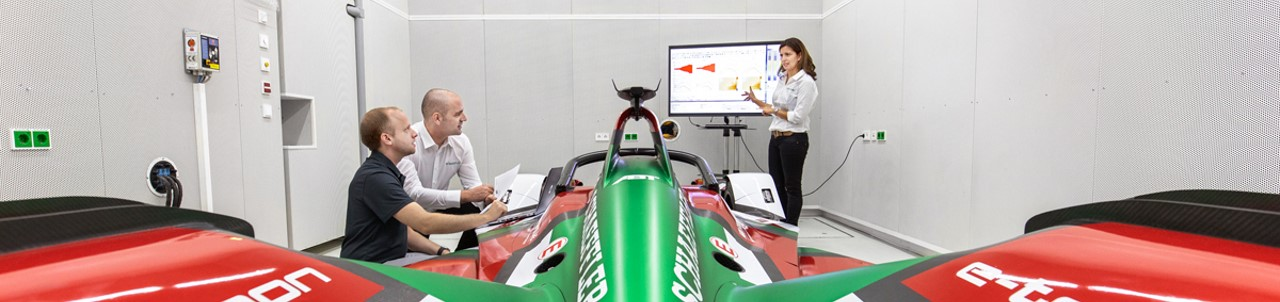
\includegraphics[width=16cm]{images/cover_sample.jpg}\\
	\vspace*{24mm}	für das 05. und 06. Theoriesemester (T3\_3101)\\
	\vspace*{3mm}		\langartikelstudiengang{} \langstudiengang{} \textbf{\studiengang}\\
	\vspace*{3mm}		\langanderdh{} \dhbw\\
	\vspace*{7mm}	\langvon\\
	\vspace*{3mm}		{\large\textbf \autor}\\
	\vspace*{7mm}	\datumAbgabe\\
\end{center}

\vfill

\flushleft
\begin{spacing}{1.2}
\begin{tabbing}
		mmmmmmmmmmmmmmmmmmmmmmmm              \= \kill
		\textbf{\langdbbearbeitungszeit} \> \zeitraum\\
		\textbf{\langdbmatriknr, \langdbkurs} \> \matrikelnr, \kurs\\
		\textbf{\langdbfirma} \> \firma\\
								\> \firmenort\\
		\textbf{\langdbgutachter}              \>  \gutachter\\
		\textbf{Kooperation}               \>  CURE Mannheim e.V.; Team Suspension\\
		\>  Coblitzallee 1-9, 68163 Mannheim\\
%		\> Team Suspension\\
		
\end{tabbing}
\end{spacing}
% \vspace{1cm}

\vspace{1cm}
\restoregeometry
\end{titlepage}
	\end{spacing}
	\newpage

	% stellt Abstand vor Kapitelüberschriften ein
	\RedeclareSectionCommand[beforeskip=\kapitelabstand         ]{chapter}
	\newgeometry{left=4cm,right=2.5cm,top=2.5cm,bottom=2.5cm}

	\pagenumbering{Roman}
	\clearpairofpagestyles
	\ohead[]{\headmark}				% Kopfzeile außen immer mit Headmark versehen
	\automark[section]{chapter}		% Headmark bestehend aus Kolumnentitel
	\ofoot[\pagemark]{\pagemark}	% Fußzeile mit Seitenzahl außen
	\renewcommand*\chapterpagestyle{plain.scrheadings}
	% \renewcommand*\partpagestyle{plain.scrheadings}		%Bei Verwendung von Parts als Überschriftenebene: Setzen des Pagestyles global
    
    \setcounter{page}{2}
	% Sperrvermerk
	%!TEX root = ../main.tex

% \newgeometry{left=2.5cm,right=2.5cm,top=2.5cm,bottom=2.5cm}

% Sperrvermerk direkt hinter Titelseite

\addchap*{\langsperrvermerk}
\thispagestyle{empty}

\vfill

\begin{figure}[H]
    \centering
    \href{https://www.curemannheim.de}{
\includegraphics[height=5cm]{images/essential/firmenlogo.png}}
\end{figure}
\vspace*{2cm}

\iflang{de}{
Der Inhalt dieser Bachelorarbeit darf weder als Ganzes noch in Auszügen Personen außerhalb des Prüfungsprozesses und des Evaluationsverfahrens zugänglich gemacht werden, sofern keine anders lautende Genehmigung von CURE vorliegt.\\

\vspace*{1cm}
Insbesondere ist eine Weitergabe an Wettbewerber von CURE oder eine Veröffentlichung, auch auszugsweise, nicht gestattet.\\

\vspace*{1cm}
Ausnahmen bedürfen der schriftlichen Genehmigung durch den entsprechenden Hauptabteilungsleiter von CURE.
}

\iflang{en}{%
  The {\arbeit} on hand 
  \begin{center}{\itshape{} \titel{}\/}\end{center} 
   contains internal resp.\ confidential data of {\firma}. It is intended solely for inspection by the assigned examiner, the head of the {\studiengang} department and, if necessary, the Audit Committee \langanderdh{} {\dhbw}. It is strictly forbidden
    \begin{itemize}
    \item to distribute the content of this paper (including data, figures, tables, charts etc.) as a whole or in extracts,
    \item to make copies or transcripts of this paper or of parts of it,
    \item to display this paper or make it available in digital, electronic or virtual form.
    \end{itemize}
  Exceptional cases may be considered through permission granted in written form by the author and {\firma}.
}

\vspace{4cm}

% \restoregeometry
    \newpage
	
	% Erklärung
 	%!TEX root = ../main.tex

% \newgeometry{left=2.5cm,right=2.5cm,top=2.5cm,bottom=2.5cm}

\addchap*{\langerklaerung}
\thispagestyle{empty}

\vspace*{1.5cm}

\iflang{de}{
    \begin{center}
        \begin{tabular}{| p{0.95\textwidth} |}
            \hline
            Ich versichere hiermit, dass ich meine \arbeit~mit dem Thema \glqq{\itshape \titel }\grqq~selbstständig verfasst und keine anderen als die angegebenen Quellen und Hilfsmittel benutzt habe.\\
            Ich versichere zudem, dass die eingereichte elektronische Fassung mit der gedruckten Fassung übereinstimmt.*\\
            \footnotesize{\emph{*Falls beide Fassungen gefordert sind}}\\
            \vspace{.5cm}
            Mannheim, den \datumAbgabe\\
            \vspace*{.5cm}
            \singlespacing
            \rule{7cm}{.5pt}\\
            \autor\\[12pt]
            \hline
        \end{tabular}
    \end{center}

    \vfill

    \begin{flushright}
        \begin{minipage}[]{0.8\textwidth}
            \flushright
            \textbf{Hinweis:}\\[6pt]
            In dieser \arbeit~wird aus Gründen der besseren Lesbarkeit das generische Maskulinum verwendet. Weibliche und anderweitige Geschlechteridentitäten werden dabei ausdrücklich mitgemeint, soweit dies für die Aussage erforderlich ist.
        \end{minipage}
    \end{flushright}
}


\iflang{en}{
    % Müsste man mal ausfüllen für eine englische Arbeit.
}

% \restoregeometry
 	\newpage

	% Abstract
	%!TEX root = ../main.tex

\pagestyle{empty}


\renewcommand{\abstractname}{\langabstract} % Text für Überschrift

\begin{otherlanguage}{english} % auskommentieren, wenn Abstract auf Deutsch sein soll
\begin{abstract}

\begin{description}
\item[Objektivität] soll sich jeder persönlichen Wertung enthalten
\item[Kürze] soll so kurz wie möglich sein
\item[Genauigkeit] soll genau die Inhalte und die Meinung der Originalarbeit wiedergeben
\end{description}

Diese etwa einseitige Zusammenfassung soll es dem Leser ermöglichen, Inhalt der Arbeit und Vorgehensweise
des Autors rasch zu überblicken. Gegenstand des Abstract sind insbesondere 
\begin{itemize}
\item Problemstellung der Arbeit,
\item im Rahmen der Arbeit geprüfte Hypothesen bzw. beantwortete Fragen,
\item der Analyse zugrunde liegende Methode,
\item wesentliche, im Rahmen der Arbeit gewonnene Erkenntnisse,
\item Einschränkungen des Gültigkeitsbereichs (der Erkenntnisse) sowie nicht beantwortete Fragen. 
\end{itemize}

\end{abstract}
\end{otherlanguage} % auskommentieren, wenn Abstract auf Deutsch sein soll

%%%%%%%%%%%%%%%%%%%%%%%%%%%%%%%%%%%%%%%%%%%%%%%%%%%%%%%%%%%%%%%%%%%%%%%%%%%%%%%%%%%%%%%%%%%%
\newpage
%%%%%%%%%%%%%%%%%%%%%%%%%%%%%%%%%%%%%%%%%%%%%%%%%%%%%%%%%%%%%%%%%%%%%%%%%%%%%%%%%%%%%%%%%%%%

\renewcommand{\abstractname}{\langabstract} % Text für Überschrift
\begin{abstract}

Deutsche Variante des Abstracts.

\end{abstract}
	\newpage

	% Inhaltsverzeichnis
	\begin{spacing}{1.2}
		\begingroup
			% auskommentieren für Seitenzahlen unter Inhaltsverzeichnis
			\renewcommand*{\chapterpagestyle}{empty}
			\pagestyle{empty}

			%\setcounter{tocdepth}{1}
			%für die Anzeige von Unterkapiteln im Inhaltsverzeichnis
			\setcounter{tocdepth}{2}

			%\tableofcontents
			\maintoc
			\clearpage
		\endgroup
	\end{spacing}
	\newpage
    
    \pagestyle{scrheadings}
	
	% noch ausstehende ToDo's - Liste
	% \listoftodos

	% Abkürzungsverzeichnis
 	\clearpage
 	%!TEX root = ../main.tex

%%%%%%%%%%%%%%%%%%%%%%%%%%%%%%%%%%%%%%%%%%%%%%%%%%%%%%%%%%%%%%%%
% Anmerkungen zur Verwendung:
%%%%%%%%%%%%%%%%%%%%%%%%%%%%%%%%%%%%%%%%%%%%%%%%%%%%%%%%%%%%%%%%
%
% nur verwendete Akronyme werden letztlich im Abkürzungsverzeichnis des Dokuments angezeigt
% Verwendung: 
%		\ac{Abk.}   --> fügt die Abkürzung ein, beim ersten Aufruf wird zusätzlich automatisch die ausgeschriebene Version davor eingefügt bzw. in einer Fußnote (hierfür muss in header.tex \usepackage[printonlyused,footnote]{acronym} stehen) dargestellt
%		\acs{Abk.}   -->  fügt die Abkürzung ein
%		\acf{Abk.}   --> fügt die Abkürzung UND die Erklärung ein
%		\acl{Abk.}   --> fügt nur die Erklärung ein
%		\acp{Abk.}  --> gibt Plural aus (angefügtes 's'); das zusätzliche 'p' funktioniert auch bei obigen Befehlen
%	siehe auch: http://golatex.de/wiki/%5Cacronym
%
%%%%%%%%%%%%%%%%%%%%%%%%%%%%%%%%%%%%%%%%%%%%%%%%%%%%%%%%%%%%%%%%

\addchap{\langabkverz}

\begin{acronym}[mmmmmm] %hier längstes Acro
% \begin{doublespacing}
% \setlength{\itemsep}{-\parsep}

\acro{KI}{Künstliche Intelligenz}
\acrodefplural{KI}[KIs]{Künstliche Intelligenzen}

\end{acronym}

	% Abbildungsverzeichnis
 	\clearpage
	%\addcontentsline{lof}{figure}{\listfigurename}
	\listoffigures
	
	% Tabellenverzeichnis
 	\clearpage
 	\listoftables
	
	% Formelgrößenverzeichnis
 	\clearpage
 	%!TEX root = ../main.tex

\addchap{Formelgrößen}

\begin{spacing}{1.5}
    \begin{tabbing}
        mmmmmmmm \= mmmmmmmm \= \kill
        \textbf{Symbol} \> \textbf{Einheit} \> \textbf{Beschreibung} \\ \vspace*{.5cm} \\
        $K$ \> $\mathsf{m^2}$ \> Permeabilität (Durchlässigkeit) \\
        $p_\mathsf{i}$ \> - \> Punktzahl des Kriteriums i \\
        $p_\mathsf{max}$ \> - \> maximal erreichbare Punktzahl eines Kriteriums i \\
        $p$ \> $\mathsf{\frac{W}{m^2}}$ \> Leistungsdichte \\
        $P$ \> W \> Leistung \\
        $Q$ \> $\mathsf{\frac{m^3}{s}}$ \> Durchflussrate 
    \end{tabbing}
\end{spacing}

	% Quellcodeverzeichnis
	\clearpage
	\lstlistoflistings
	
	\cleardoublepage
	\pagenumbering{arabic}
    
    \pagestyle{scrheadings}		% Kopf- und Fußzeile wie zuvor eingestellt
	
	%\setcounter{footnote}{1}	% Dont start at 2

    \pagestyle{scrheadings}
	% Inhalt
	\foreach \i in {01,02,03,04,05,06,07,08,09,...,99} {%
		\edef\FileName{content/\i kapitel}%
			\IfFileExists{\FileName}{%
				\input{\FileName}
			}
			{%
				%file does not exist
			}
	}

	\clearpage
	
    \pagenumbering{Roman}
    \setcounter{page}{21}
     
	% Literaturverzeichnis
	% \clearpage
	\printbibliography
	% \printbibliography[notkeyword=intern, nottype=patent]
	% \printbibliography[heading=subbibliography, keyword=intern, title={Interne Quellen}]
	% \printbibliography[heading=subbibliography, type=patent, title={Patentschriften}]
	% Unterverzeichnisse siehe: https://texwelt.de/fragen/7532/wie-unterteile-ich-meine-biblatex-bibliografie
    
	% sonstiger Anhang
	\cleardoublepage
	\pagenumbering{Alph}
	\appendix
	% !TeX root = ../dokumentation.tex

\appendixtoc
\renewcommand\thechapter{\Alph{chapter}}
\setcounter{chapter}{0}

% \pagebreak
% \includepdf[pages=-,scale=.9,pagecommand={}]{Aufgabenstellung.pdf} 
% PDF um 10% verkleinert einbinden --> Kopf- und Fußzeile  werden so korrekt dargestellt. Die Option `pages' ermöglicht es, eine bestimmte Sequenz von Seiten (z.B. 2-10 oder `-' für alle Seiten) auszuwählen.
% \pagebreak
%\includepdf[pages=-,scale=.8,pagecommand=\section*{A. eventGenerator.py}]{../appendix/eventGenerator.py.pdf}
%\includepdf[pages=-,scale=.8,pagecommand=\section*{B. sendEvents.py}]{../appendix/sendEvents.py.pdf}


%%%%%%%%%%%%%%%%%%%%%%%%%%%%%%%%%%%%%%%%%%%%%%%%%%%%%
\chapter{Grafiken}

%%%%%%%%%%%%%%%%%%%%%%%%%%%%%%%%%%%%%%%%%%%%%%%%%%%%%
\chapter{Tabellenwerke}

%%%%%%%%%%%%%%%%%%%%%%%%%%%%%%%%%%%%%%%%%%%%%%%%%%%%%
\chapter{Sonstiges}

% \section{Datenblatt: Titan Grade 5 (3.7165; Ti6Al4V) - HWN Titan GmbH \cite{HWN.2022}}
% \label{section:Titandatenblatt}
% \begin{figure}[h]
%     \centering
%     \includegraphics[width=.73\textwidth]{images/appendix/DatenblattTitanGrade5.png}
% \end{figure}
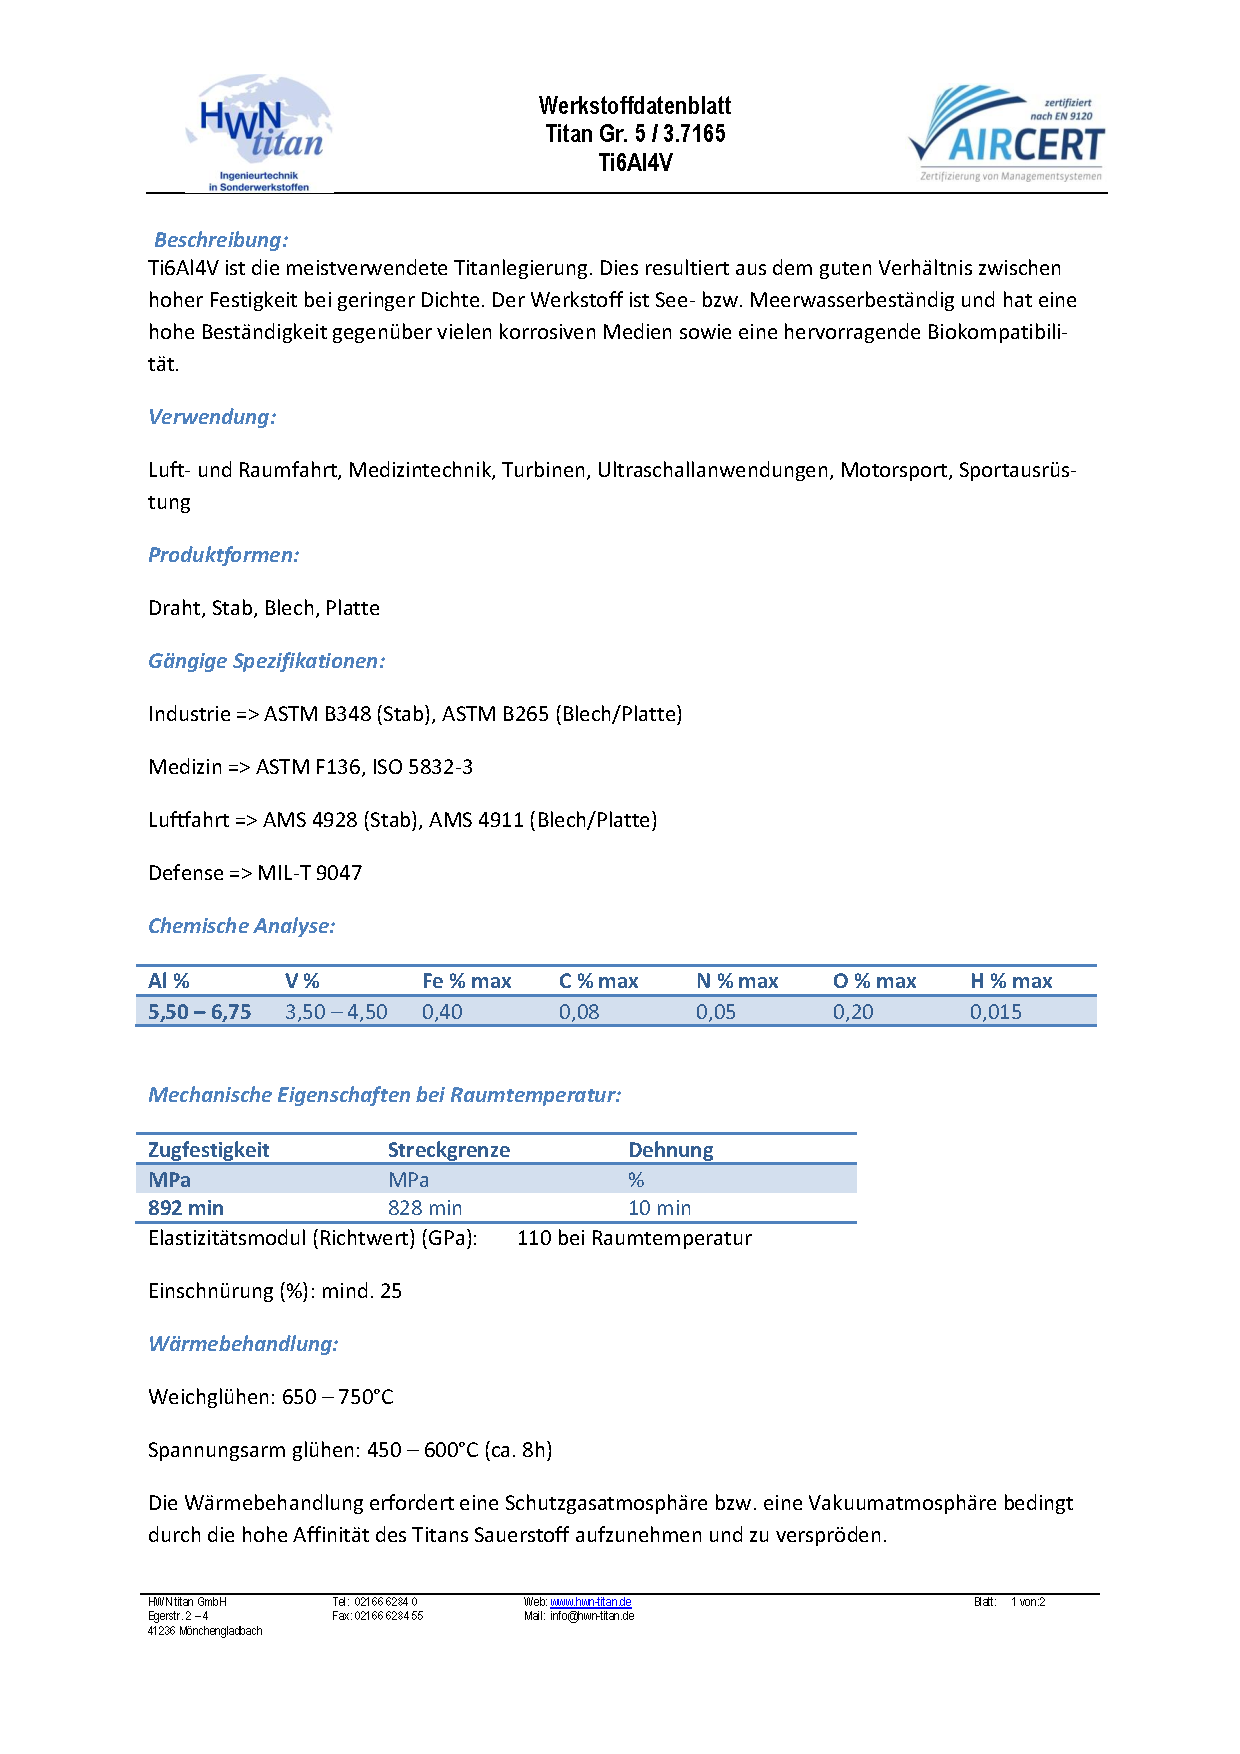
\includepdf[pages=1,scale=.7,pagecommand=\section{Datenblatt: Titan Grade 5 (3.7165; Ti6Al4V) - HWN Titan GmbH}\label{section:Titandatenblatt}]{images/appendix/titan-grade-5-werkstoffdatenblatt.pdf}

\end{document}
